\documentclass[12pt,a4paper]{article}
\usepackage[UTF8]{ctex}
\usepackage{amsmath,amssymb}
\usepackage{listings}
\usepackage{xcolor}
\usepackage{hyperref}
\usepackage{geometry}
\usepackage{graphicx}
\geometry{margin=2.5cm}

\lstdefinestyle{python}{
  language=Python,
  basicstyle=\ttfamily\small,
  keywordstyle=\color{blue}\bfseries,
  commentstyle=\color{gray},
  stringstyle=\color{red},
  showstringspaces=false,
  breaklines=true,
  frame=single,
  backgroundcolor=\color{gray!10}
}

\title{Quantum Counting / 量子计数}
\author{QuoNic}
\date{}

\begin{document}
\maketitle

\begin{center}
\textbf{Algorithms / 算法} | 难度：中级 | 预计时间：15 分钟
\end{center}

\tableofcontents
\newpage

\section{为什么需要？}

量子计数用于计算满足条件的解的数量，是 Grover 搜索的推广。

\subsection{经典局限}
\b\begin{itemize}
  \item 经典计数需要遍历所有元素
  \item 对于 $N$ 个元素，经典需要 $O(N)$ 次查询
\end{itemize}

\subsection{量子优势}
\b\begin{itemize}
  \item 量子计数只需要 $O(\sqrt{N})$ 次查询
  \item 可以估计解的数量而不需要找到解
  \item 是量子算法设计的重要工具
\end{itemize}

\subsection{实际应用}
\b\begin{itemize}
  \item 数据库计数
  \item 优化问题（估计解空间大小）
  \item 量子算法设计
\end{itemize}

\section{快速上手}

\begin{lstlisting}[style=python]
from quonic.algorithms import quantum_counting

# Count solutions in 2-qubit space
result = quantum_counting(n_qubits=2, n_solutions=1)
print(f"Estimated count: {result.count}")
\end{lstlisting}

\textbf{预期输出}：
\begin{verbatim}
Estimated count: 1
\end{verbatim}

\section{原理详解}

\subsection{电路图}

\begin{center}
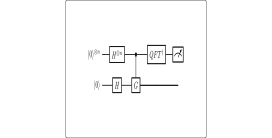
\includegraphics[width=0.7\textwidth]{../../images/quantum_counting_circuit.svg}
\end{center}

\subsection{数学推导}

量子计数结合了 Grover 搜索和量子相位估计：
\begin{equation}
G = (2|s\rangle\langle s| - I)O
\end{equation}

其中 $O$ 是 Oracle，$|s\rangle$ 是均匀叠加态。

通过 QPE 估计 $G$ 的本征值，可以推算出解的数量：
\begin{equation}
M = N \sin^2(\theta/2)
\end{equation}

\subsection{几何解释}

量子计数在 Bloch 球上估计 Grover 算子的旋转角度，从而推算解的数量。

\section{代码详解}

\begin{lstlisting}[style=python]
from quonic.algorithms import quantum_counting

# quantum_counting(n_qubits, n_solutions)
# n_qubits: number of qubits
# n_solutions: actual number of solutions (for verification)
result = quantum_counting(n_qubits=2, n_solutions=1)

# result.count: estimated number of solutions
# result.phase: estimated phase
print(f"Count: {result.count}")
\end{lstlisting}

\section{进阶用法}

\subsection{场景 1：不同解数量}

\begin{lstlisting}[style=python]
# Count different numbers of solutions
for n in range(1, 5):
    result = quantum_counting(n_qubits=3, n_solutions=n)
    print(f"Actual: {n}, Estimated: {result.count}")
\end{lstlisting}

\section{适用场景}

\subsection{数据库计数}

量子计数可以高效计算满足条件的记录数量。

\subsection{优化问题}

量子计数可以估计解空间的大小。

\section{常见问题}

\subsection{量子计数和 Grover 搜索有什么区别？}

Grover 搜索找到一个解，量子计数估计解的数量。

\subsection{量子计数的精度如何？}

精度取决于控制量子比特的数量。更多的控制量子比特提供更高的精度。

\section{学习路径}

\subsection{前置知识}
\b\begin{itemize}
  \item Grover 搜索
  \item 量子相位估计（QPE）
  \item 量子傅里叶变换（QFT）
\end{itemize}

\subsection{继续学习}
\b\begin{itemize}
  \item 振幅放大
  \item 量子优化
  \item 量子机器学习
\end{itemize}

\section{完整示例代码}

\subsection{示例 1：基本量子计数}

\begin{lstlisting}[style=python]
from quonic.algorithms import quantum_counting

result = quantum_counting(n_qubits=2, n_solutions=1)
print(f"Count: {result.count}")
\end{lstlisting}

\

\section{下载}

\begin{itemize}
  \item [quantum_counting.py](https://github.com/ChrisLee0721/QuoNic/blob/main/examples/quantum_counting/quantum_counting.py)
\end{itemize}

\end{document}
